\documentclass[11pt]{article}
\usepackage{spikey}
\usepackage{amsmath}
\usepackage{amssymb}
\usepackage{soul}
\usepackage{float}
\usepackage{graphicx}
\usepackage{hyperref}
\usepackage{xcolor}
\usepackage{chngcntr}
\usepackage{centernot}
\usepackage[shortlabels]{enumitem}

\usepackage[margin=1truein]{geometry}

\title{Forecasting and Time Series Econometrics \\ ECO374 Winter 2019}
\date{\today}
\author{Tianyu Du}

\counterwithin{equation}{section}
\counterwithin{theorem}{section}
\counterwithin{lemma}{section}
\counterwithin{corollary}{section}
\counterwithin{proposition}{section}
\counterwithin{remark}{section}
\counterwithin{example}{section}
\counterwithin{figure}{section}


\begin{document}
	\maketitle
	\tableofcontents
	
	\section{Introduction and Statistics Review}
		\begin{definition}
			Given random variable $X$, the $k^{th}$ \textbf{non-central moment} is defined as
			\begin{equation}
				\expect{X^k}
			\end{equation}
		\end{definition}
		
		\begin{definition}
			Given random variable $X$, the $k^{th}$ \textbf{central moment} is defined as
			\begin{equation}
				\expect{(X - \expect{X})^k}
			\end{equation}
		\end{definition}
		
		\begin{remark}
			Moments of order higher than a certain $k$ may not exist for certain distribution.
		\end{remark}
		
		\begin{definition}
			Given the \textbf{joint density} $f(X,Y)$ of two \emph{continuous} random variables, the \textbf{conditional density} of random $Y$ conditioned on $X$ is 
			\begin{equation}
				f_{Y|X}(y|x) = \frac{f_{Y,X}(y,x)}{f_X(x)}
			\end{equation}
		\end{definition}
		
		\begin{definition}
			Given discrete variables $X$ and $Y$, the \textbf{conditional density} of $Y$ conditioned on $X$ is defined as 
			\begin{equation}
				P(Y=y|X=x) = \frac{P(Y=y \land X=x)}{P(X=x)}
			\end{equation}
		\end{definition}
		
		\begin{assumption} Assumptions on linear regression on time series data:
			\begin{enumerate}[(i)]
				\item \textbf{Linearity}
					\begin{equation}
						Y = \beta_0 + \beta_1 X_1 + \dots + \beta_k X_k + u
					\end{equation}
				\item \textbf{Zero Conditional Mean}
					\begin{equation}
						\expect{u|X_1, X_2, \dots, X_k} = 0
					\end{equation}
				\item \textbf{Homoscedasitcity}
					\begin{equation}
						\var{u|X_1, X_2, \dots, X_k} = \sigma^2_u
					\end{equation}
				\item \textbf{No Serial Correlation}
					\begin{equation}
						Cov(u_t, u_s) = 0\ \forall t \neq s \in \Z
					\end{equation}
				\item \textbf{No Perfect Collinearity}
				\item \textbf{Sample Variation in Regressors}
					\begin{equation}
						\var{X_j} > 0\ \forall j
					\end{equation}
			\end{enumerate}
		\end{assumption}
		
		\begin{theorem}[Gauss-Markov Theorem]
			Under assumptions 1.1, the OLS estimators $\hat{\beta}_j$ are \emph{best linear unbiased estimators} of the unknown population regression coefficients $\beta_j$.
		\end{theorem}
		
		\begin{remark}
			The \emph{no serial correlation} assumption is typically not satisfied for time series data. And the \emph{linearity} assumption is also too restrictive for time series featuring complex dynamics. Hence, for time series data we typically use other models than linear regression with OLS.
		\end{remark}
		
	\section{Statistics and Time Series}
		\subsection{Stochastic Processes}
		\begin{definition}[1.1]
			A \textbf{stochastic process} (or \textbf{time series process}) is a family (collection) random variables indexed by $t \in \mc{T}$ and defined on some given probability space $(\Omega, \mc{F}, P)$.
			\begin{equation}
				\{Y_t\} = Y_1, \dots, Y_T
			\end{equation}
		\end{definition}
		
		\begin{definition}[1.2]
			The function $t \to y_t$ which assigns to each point in time $t \in \mc{T}$ the realization of the random variable $Y_t$, $y_t$ is called a \textbf{realization} or a \textbf{trajectory} or an \textbf{outcome} of the stochastic process.
		\end{definition}
		
		\begin{definition}
			An \emph{outcome} of a stochastic process 
			\begin{equation}
				\{y_t\} = y_1, \dots, y_T
			\end{equation}
			is a \textbf{time series}.
		\end{definition}
		
		\begin{definition}[1.3]
			A \textbf{time series model} or a \textbf{model} for the observations (data), $\{y_t\}$, is a specification of the \emph{joint distribution} of $\{Y_t\}$ for which $\{y_t\}$ is a realization.
		\end{definition}
		
		\begin{assumption}
			The \textbf{ergodicity} assumption requires the observations cover in principle all possible events.
		\end{assumption}
		
		\begin{definition}
			A stochastic process $\{Y_t\}$ is \textbf{first order strongly stationary} if all random variables $Y_t \in \{Y_t\}$ has the \emph{same probability density function}.
		\end{definition}
		
		\begin{definition}[1.7]
			A stochastic process $\{Y_t\}$ is \textbf{strictly stationary} if for all $h, n \geq 1$, $(X_1,\dots,X_n)$ and $(X_{1+h}, \dots, X_{n+h}$ have the same distribution.
		\end{definition}
		
		\begin{definition}
			A stochastic process $\{Y_t\}$ is \textbf{first order weakly stationary} if
			\begin{equation}
				\forall t \in \mc{T},\ \mu_{Y_t} \equiv \expect{Y_t} = \bar{\mu}
			\end{equation}
		\end{definition}
		
		\begin{definition}
			A stochastic process $\{Y_t\}$ is \textbf{second order weakly stationary}, or \textbf{covariance stationary} if all random variables $\{Y_t\}$ have the same mean and variance. And the covariances do not depend on $t$.
			That's, for all $t \in \mc{T}$,
			\begin{enumerate}[(i)]
				\item $\expect{Y_t} = \mu\ \forall t$
				\item $\var{Y_t} = \sigma^2 < \infty\ \forall t$
				\item $Cov(Y_t, Y_s) = Cov(Y_{t+r}, Y_{s+r})\ \forall t,s,r\in \Z$
			\end{enumerate}
		\end{definition}
		
		\subsection{Auto-correlations}
		
		\begin{definition}
			Let $\{Y_t\}$ be a stochastic process with $\var{Y_t} < \infty\ \forall t \in \mc{T}$, the \textbf{auto-covariance function} is defined as
			\begin{gather}
				\gamma_Y(t, s) \equiv Cov(Y_t, Y_s) \\
				= \expect{(Y_t - \expect{Y_t})(Y_s - \expect{Y_s})} \\
				= \expect{Y_t Y_s} - \expect{Y_t} \expect{Y_s}
			\end{gather}
		\end{definition}
		
		\begin{lemma}
			If $\{Y_t\}$ is stationary, then the auto-covariance function does not depend on specific time point $t$. We can write the $h \in \Z$ degree auto-covariance as 
			\begin{equation}
				\gamma_Y(h) \equiv \gamma_X(t, t+h)\ \forall t \in \mc{T}
			\end{equation}
		\end{lemma}
	
		\begin{proposition}
			By the symmetry of covariance, 
			\begin{equation}
				\gamma_Y(h) = \gamma_Y(-h)
			\end{equation}
		\end{proposition}
		
		\begin{definition}
			The \textbf{auto-correlation coefficient} of order $k$ is given by
			\begin{equation}
				\rho_{Y_t, Y_{t-k}} = \frac{Cov(Y_t, Y_{t-k})}{\sqrt{\var{Y_t}}\sqrt{\var{Y_{t-k}}}}
			\end{equation}
		\end{definition}
		
		\begin{definition}
			Let $\{Y_t\}$ be a \emph{stationary process} and the \textbf{auto-correlation function} (ACF) is a mapping from \emph{order} of auto-correlation coefficient to the coefficient $\rho_Y: k \to \rho_{Y_t, Y_{t-k}}$, defined as
			\begin{equation}
				\rho_Y(k) \equiv \frac{\gamma(k)}{\gamma(0)} = corr(Y_{t + k}, Y_t)
			\end{equation}
		\end{definition}
		
		\begin{proposition}
			Note that 
			\begin{equation}
				\rho_k = \rho_{-k} = \rho_{|k|}
			\end{equation}
			so the ACF for stationary process can be simplified to a mapping 
			\begin{equation}
				\rho: k \to \rho_{|k|}
			\end{equation}
		\end{proposition}
		
		\begin{remark}
			Strong stationarity is difficult to test so we will focus on weak stationarity only.
		\end{remark}
		
		\begin{proposition}
			For a non-stationary stochastic process $\{Y_t\}$, $\{\Delta Y_t\}$ becomes \emph{first order weakly stationary} and $\{\Delta \log(Y_t)\}$ becomes \emph{second order weakly stationary}.
			\begin{figure}[h]
				\centering
				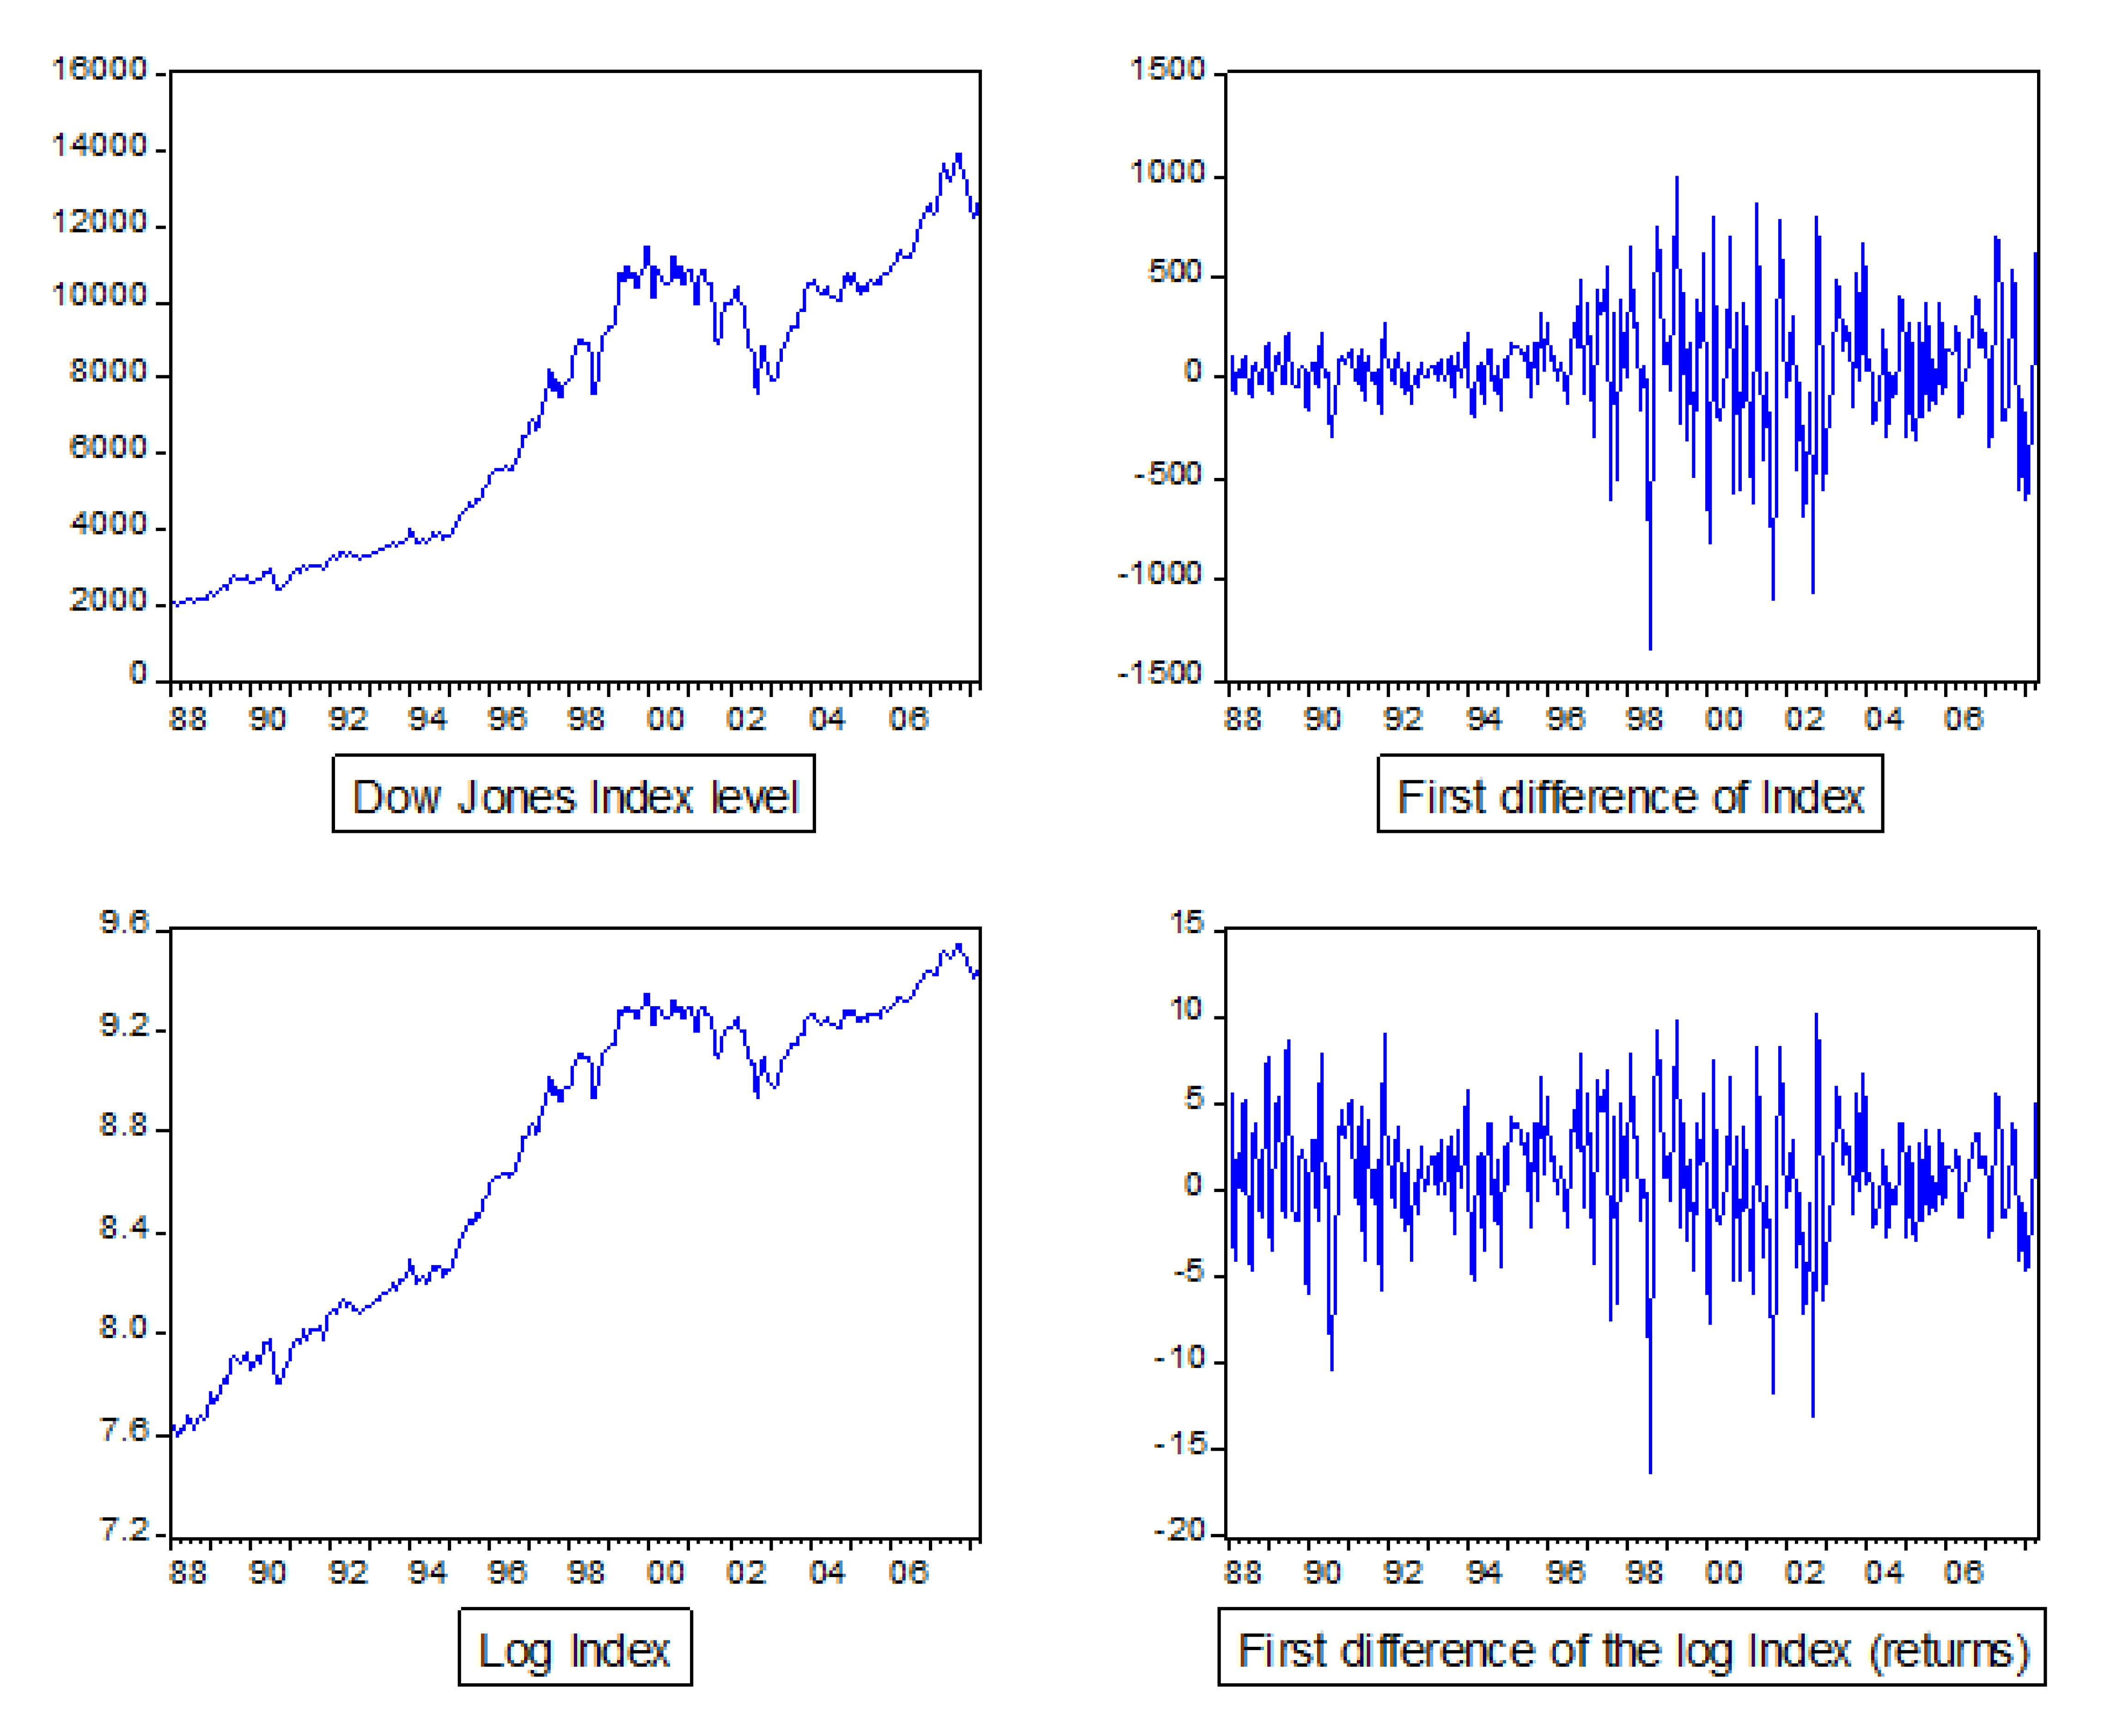
\includegraphics{figures/2_1}
			\end{figure}
		\end{proposition}
		
		\begin{definition}[1.8]
			A stochastic process $\{Y_t\}$ is called a \textbf{Gaussian process} if all \emph{finite} dimensional distribution from the process are multivariate normally distributed. That's
			\begin{gather}
				\forall n \in \Z_{>0},\ \forall (t_1, \dots, t_n) \in \mc{T}^n, (Y_{t_1}, \dots, Y_{t_n}) \sim \mc{N}(\bs{\mu}, \Sigma)
			\end{gather}
		\end{definition}
		
		\begin{notation}
			Consider the problem of forecasting $Y_{T+1}$ from observations $\{Y_t\}_{t=1}^{T}$, the \emph{best linear predictor} is denoted as
			\begin{equation}
				\mathbb{P}_T Y_{T+1} = \sum_{i=1}^{T} a_i L^i Y_{T+1}
			\end{equation}
			And $Y_{T+1}$ can be expressed as
			\begin{equation}
				Y_{T+1} = \mathbb{P}_T Y_{T+1} + Z_{T+1}
			\end{equation}
			where $Z_{T+1}$ denotes the forecast error which is \emph{uncorrelated} with $X_T, \dots, X_1$.
		\end{notation}
		
		\begin{definition}[3.3]
			The \textbf{partial auto-correlation function} (PACT) $\alpha(h)$ with $h \in \Z_{\geq 0}$ of a \emph{stationary} process is defined as 
			\begin{gather}
				\alpha(0) = 1 \\
				\alpha(1) = corr(Y_2, Y_1) = \rho(1) \\
				\alpha(h) = corr\Big(Y_{h+1} - \mathbb{P}(Y_{h+1}|1,Y_2, \dots, Y_h), X_1 - \mathbb{P}(Y_1|1,Y_2,\dots,Y_h)\Big)
			\end{gather}
		\end{definition}
		
		\begin{remark}[Interpretation of PACF] partial auto-correlation $r_k$ only measures correlation between two variables $Y_t$ and $Y_{t+k}$ while controlling $(Y_{t+1}, \dots, Y_{t+k-1})$.
		\end{remark}
		
		\begin{remark}Properties of ACF and PACF
			\begin{table}[h]
				\centering
				\begin{tabular}{l|c|c}
					processes & ACF & PACF \\
					\hline
						$AR(p)$ & 
						\begin{tabular}{@{}c@{}}Declines exponentially \\(monotonic or oscillating) to zero\end{tabular} & 
						$\alpha(h) = 0\ \forall h > p$\\
					\hline
						$MA(q)$ &
						$\rho(h) = 0\ \forall h > q$ &
						\begin{tabular}{@{}c@{}}Declines exponentially \\(monotonic or oscillating) to zero\end{tabular}
				\end{tabular}
			\end{table}
		\end{remark}
		
		\paragraph{Test for Auto-correlation}To test single auto-correlation with 
		\begin{equation}
			H_0: \rho_k = 0
		\end{equation}
		we can use usual t-statistic. While testing the joint hypothesis
		\begin{equation}
			H_0: \rho_1 = \rho_2 = \dots = \rho_k = 0
		\end{equation}
		we are using the \textbf{Ljung-Box Q-statistic}:
		\begin{equation}
			Q_k = T(T+1) \sum_{j=1}^k \frac{\hat{\rho}_j^2}{T-j} \sim \chi_k^2
		\end{equation}
	
	\section{Forecasting Tools}
	\subsection{Information Set}
		\begin{definition}
			For stochastic process $\{Y_t\}$, the \textbf{information set} $I_t$ is the \emph{known time series} up to time $t$.
		\end{definition}
		
		\begin{definition}
			A \textbf{forecast} $f_{t,h}$ the image of a \emph{time series model} $g$ under given information set $I_t$. Specifically,
			\begin{equation}
				f_{t,h} = g(I_t) \in \Omega
			\end{equation}
		\end{definition}
	\subsection{Forecast Horizon}
		\begin{remark}
			\emph{Covariance stationary} processes are \textbf{short-memory processes}. More recent observation contains information far more relevant for the future than older information.
		\end{remark}
		
		\begin{remark}
			\emph{Non-stationary} processes are \textbf{long-memory processes} and older information is as relevant for the forecast as more recent information.
		\end{remark}
		\subsubsection{Forecasting Environments: \emph{Recursive}}
			\begin{enumerate}[(i)]
				\item \emph{Updating} with \emph{flexible} information set.
				\item Advantageous if model is \emph{stable over time}.
				\item Not robust to \emph{structural break}. 
			\end{enumerate}
			\begin{figure}[H]
				\centering
				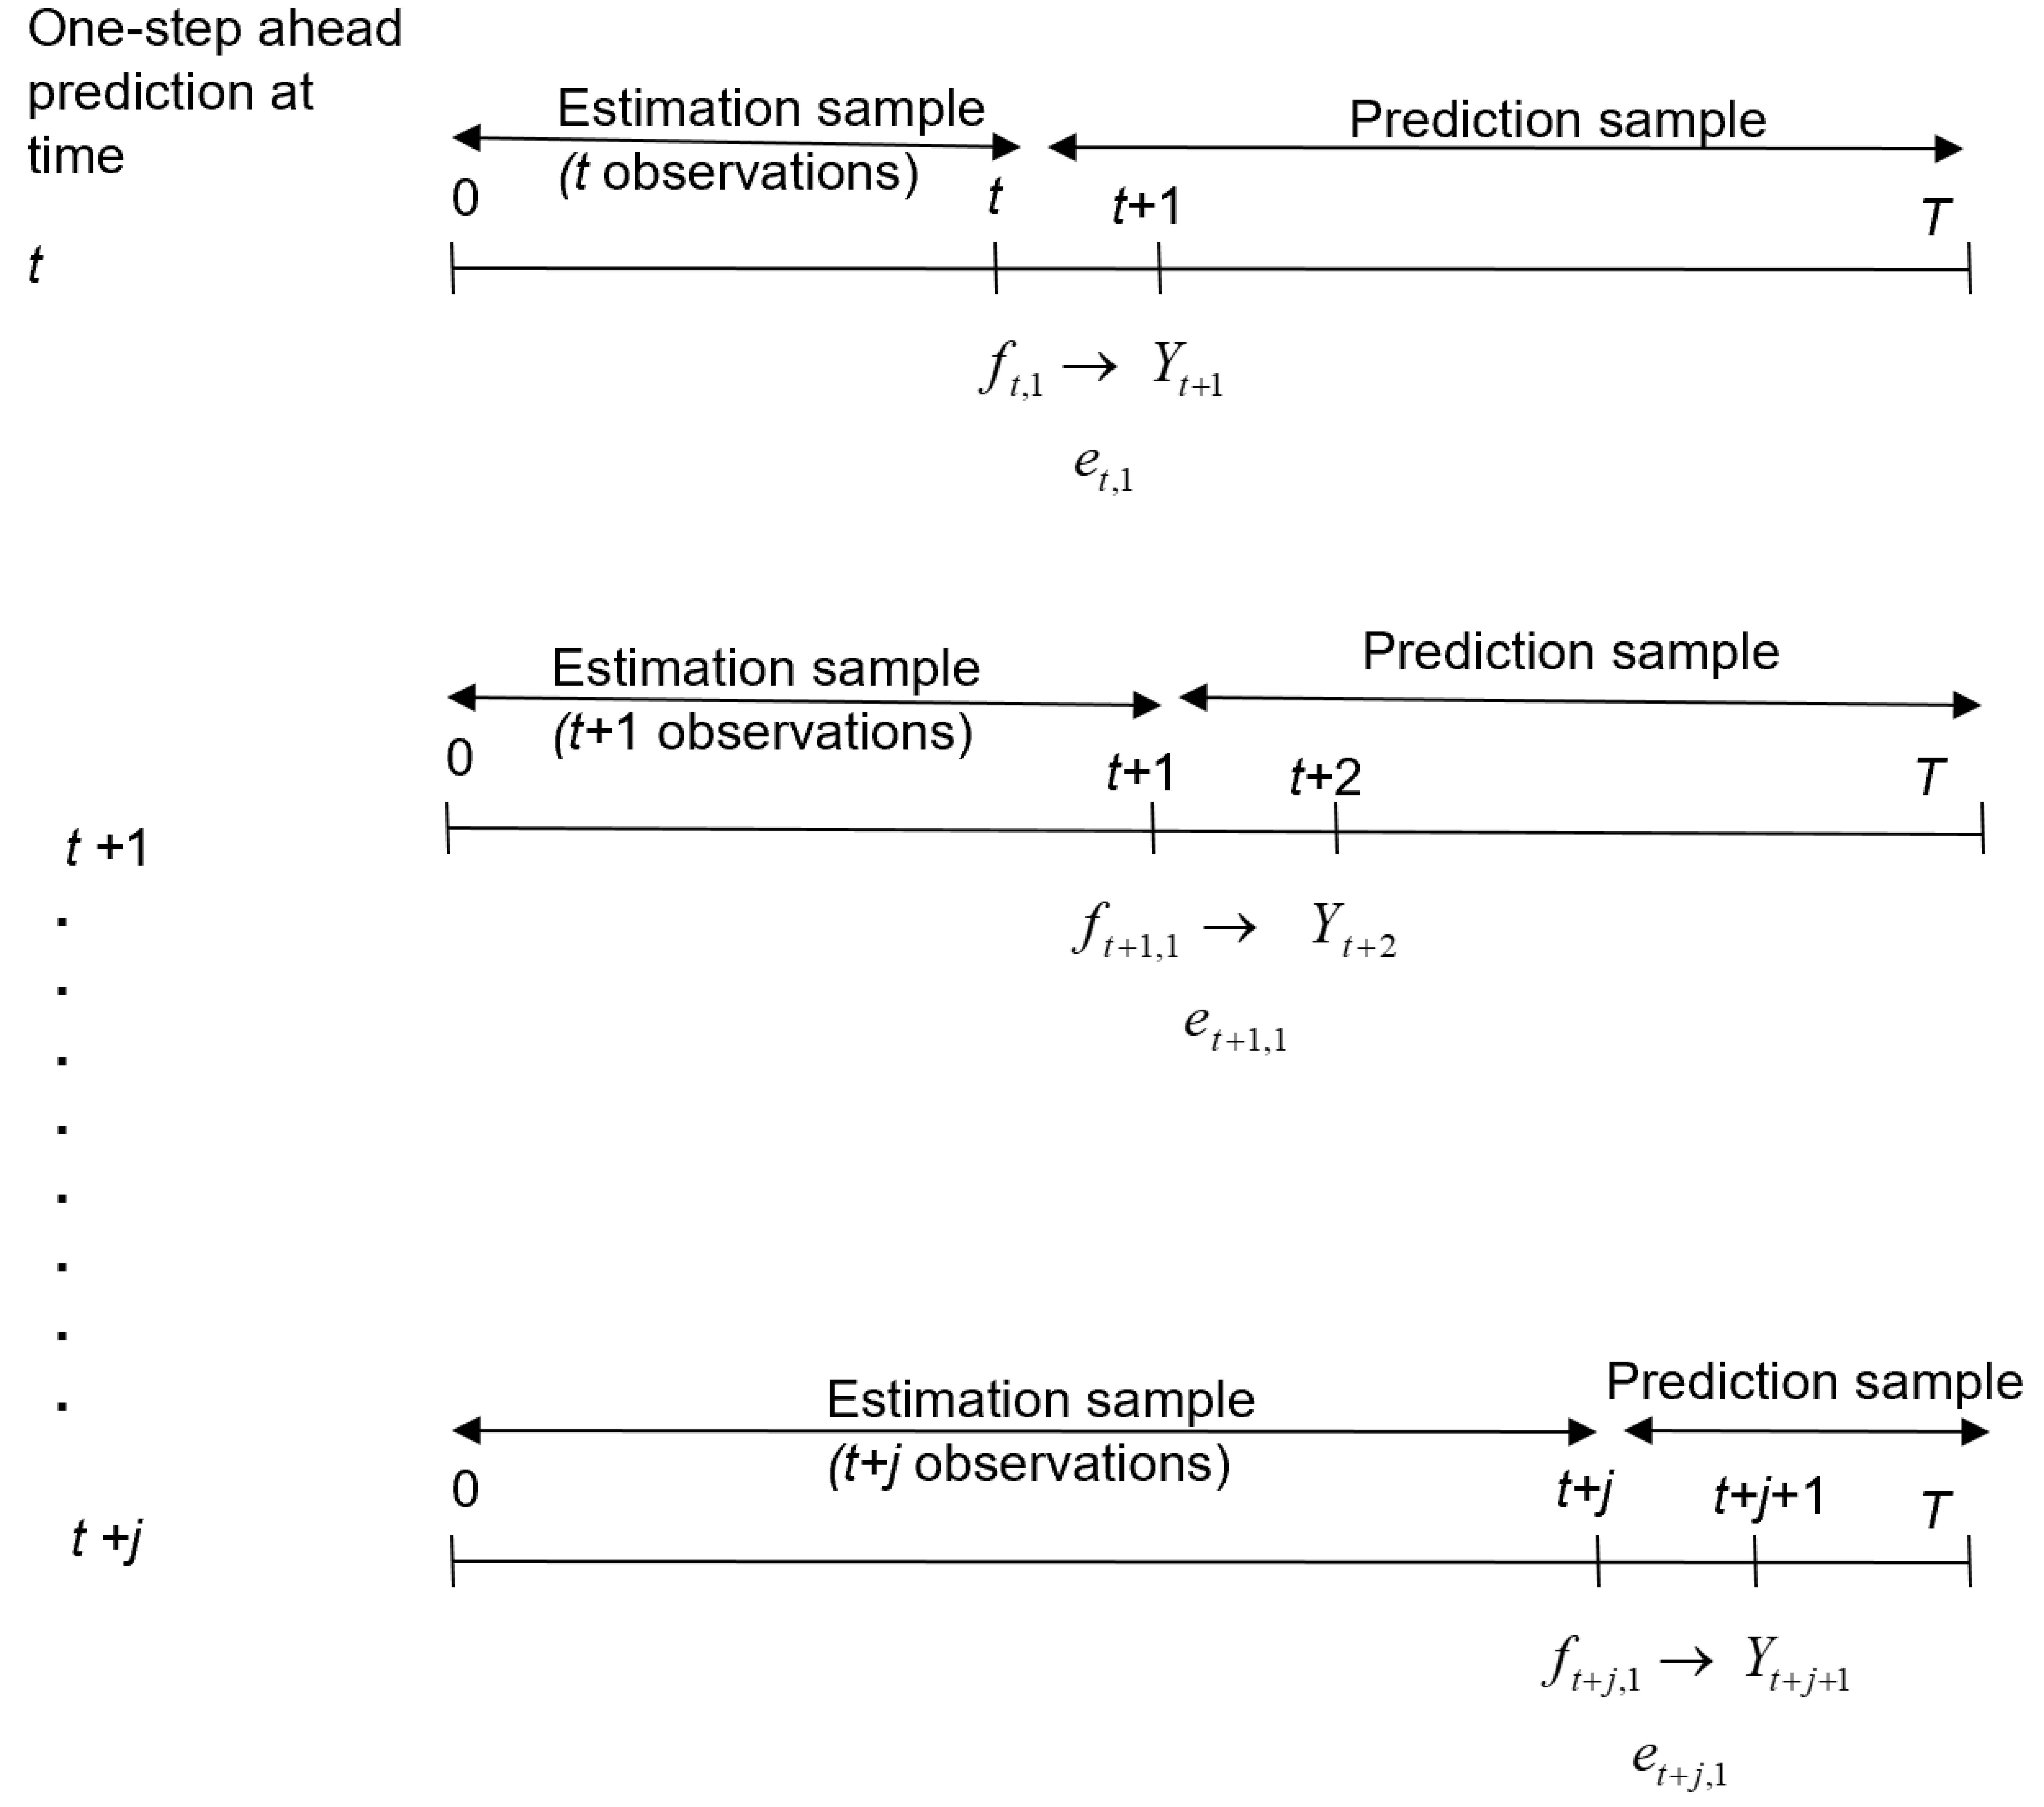
\includegraphics[width=0.5\linewidth]{figures/recursive_forecast}
				\caption{Recursive Forecasting Scheme}
			\end{figure}
		\subsubsection{Forecasting Environments: \emph{Rolling}}
			\begin{enumerate}[(i)]
				\item \emph{Updating} with \emph{fixed-size} information set.
				\item Robust against \emph{structural breaks}.
				\item Not fully exploit information available.
			\end{enumerate}
			\begin{figure}[H]
				\centering
				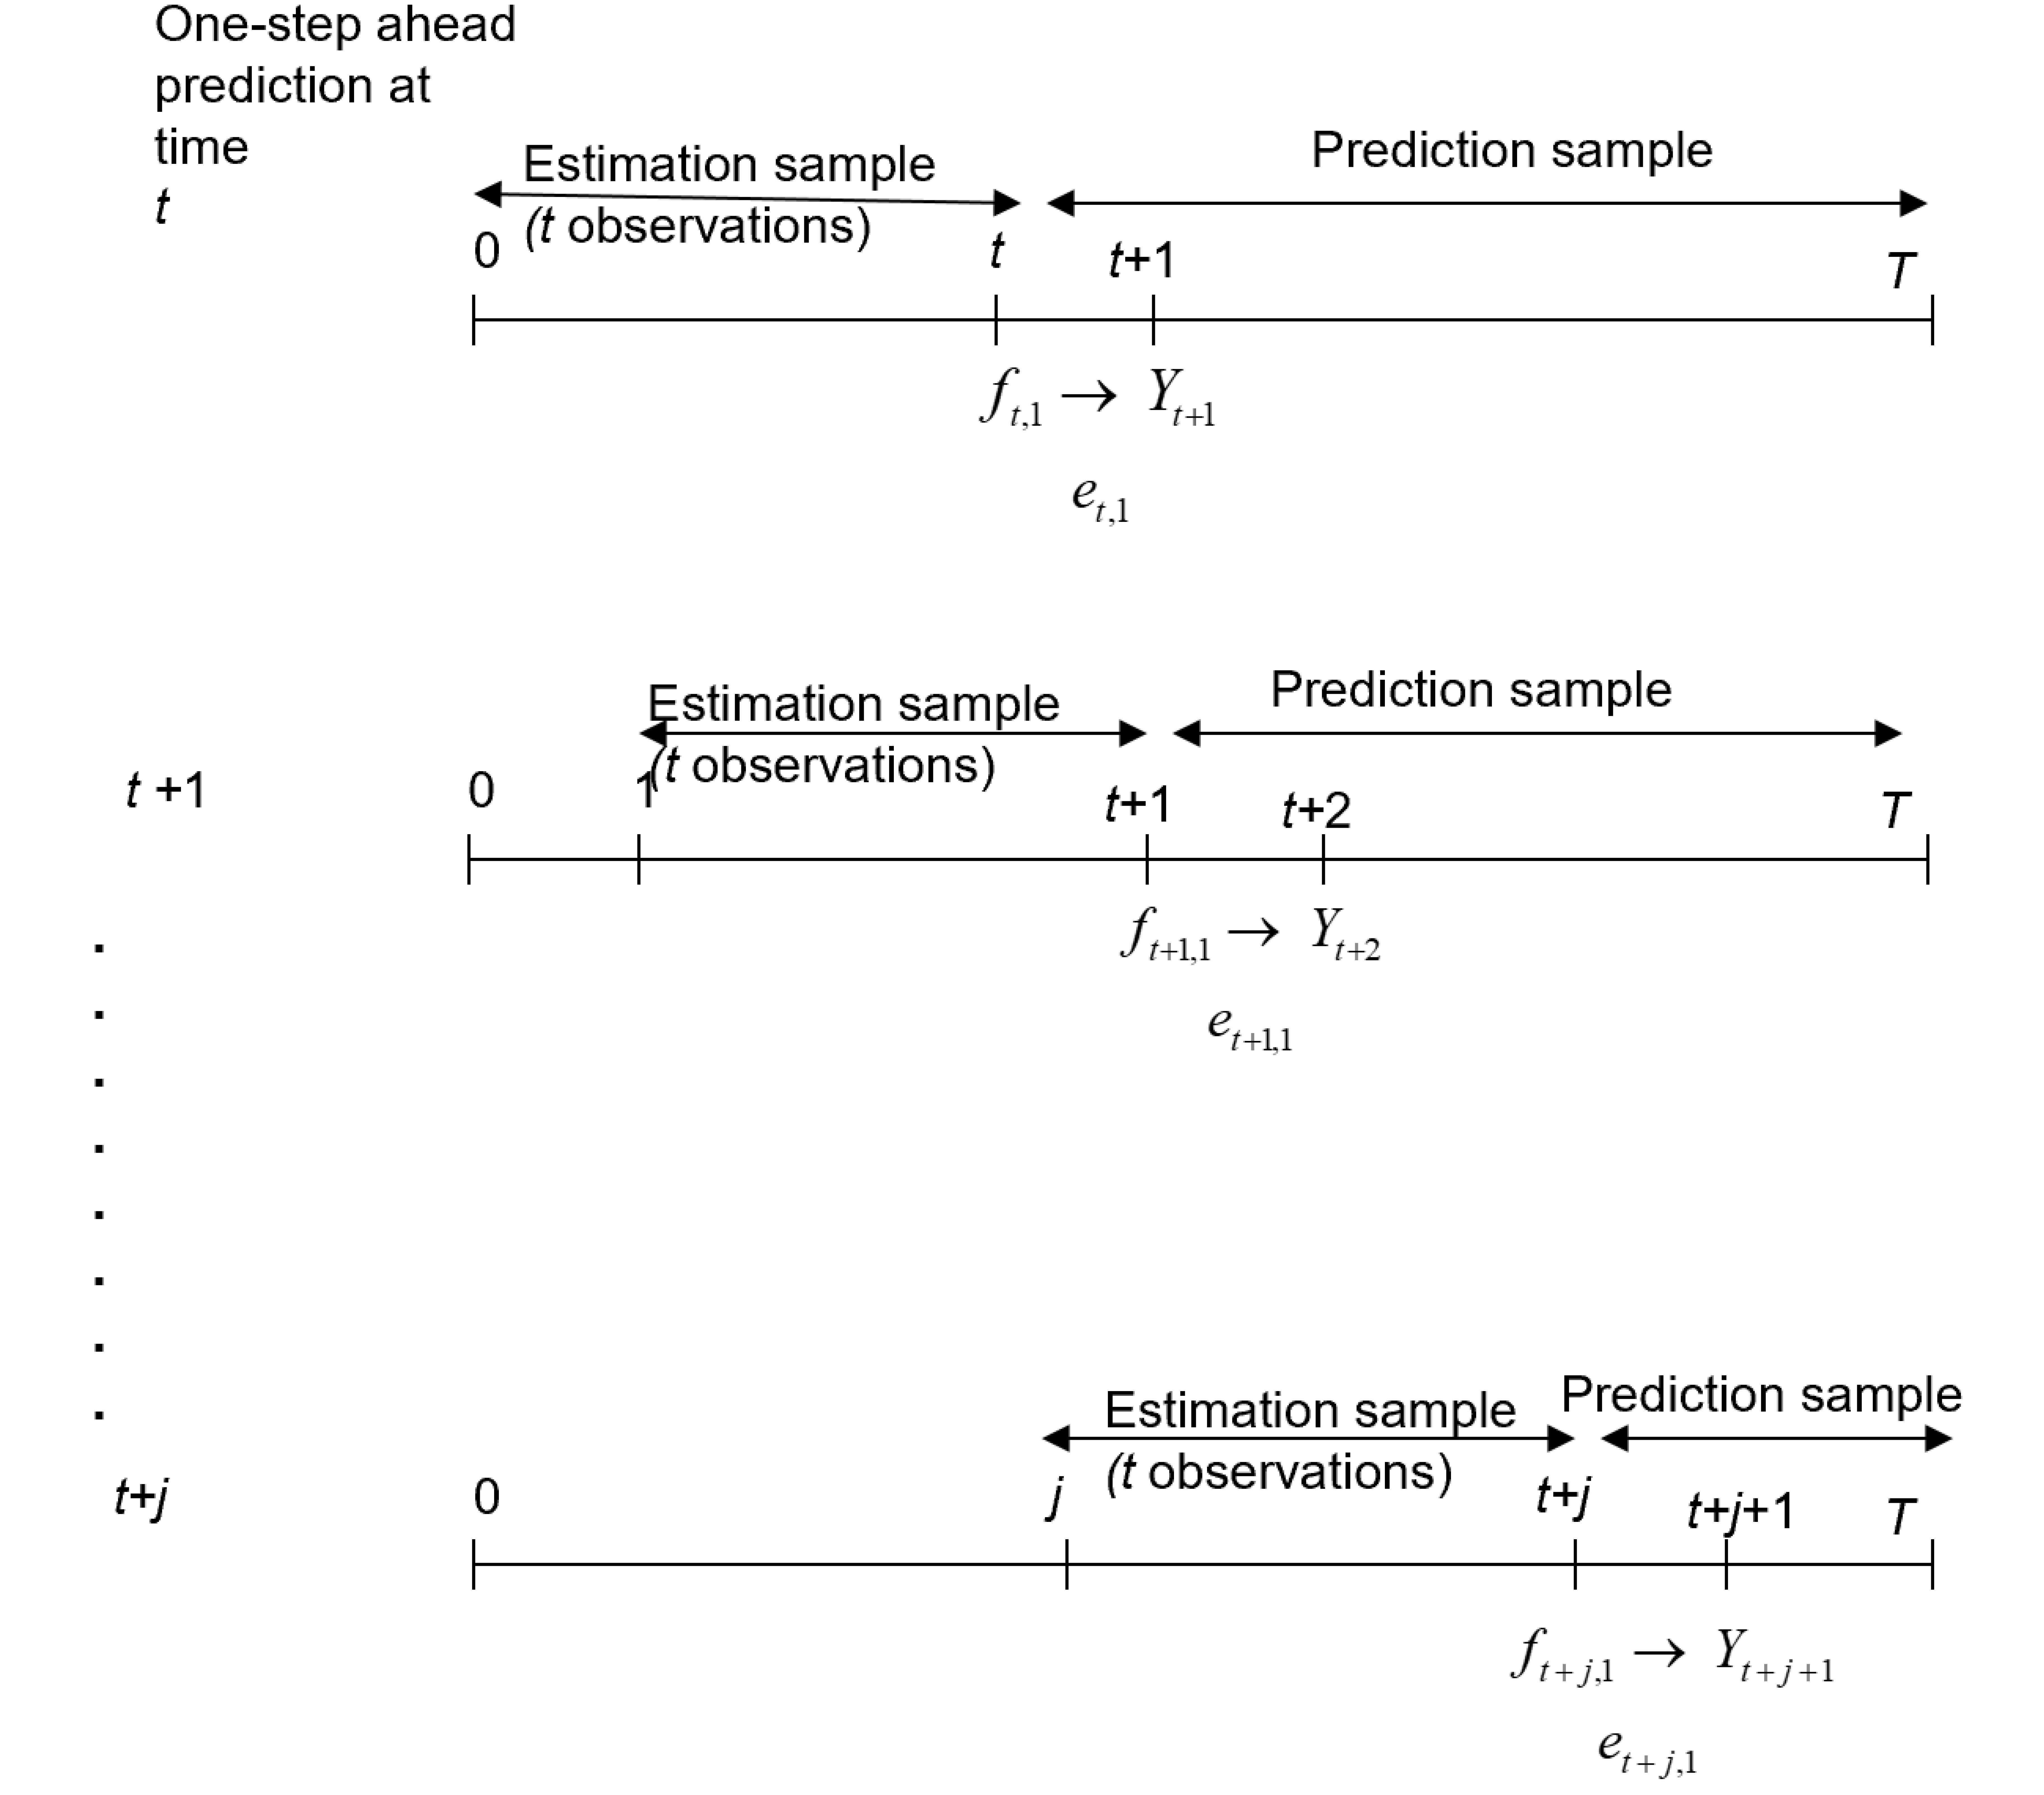
\includegraphics[width=0.5\linewidth]{figures/rolling_forecast}
				\caption{Rolling Forecasting Scheme}
			\end{figure}
		\subsubsection{Forecasting Environments: \emph{Fixed}}
			\begin{enumerate}[(i)]
				\item \emph{One estimation} and forecast with \emph{fixed-size but updated} information set.
				\item Computationally cheap.
			\end{enumerate}
			\begin{figure}[H]
				\centering
				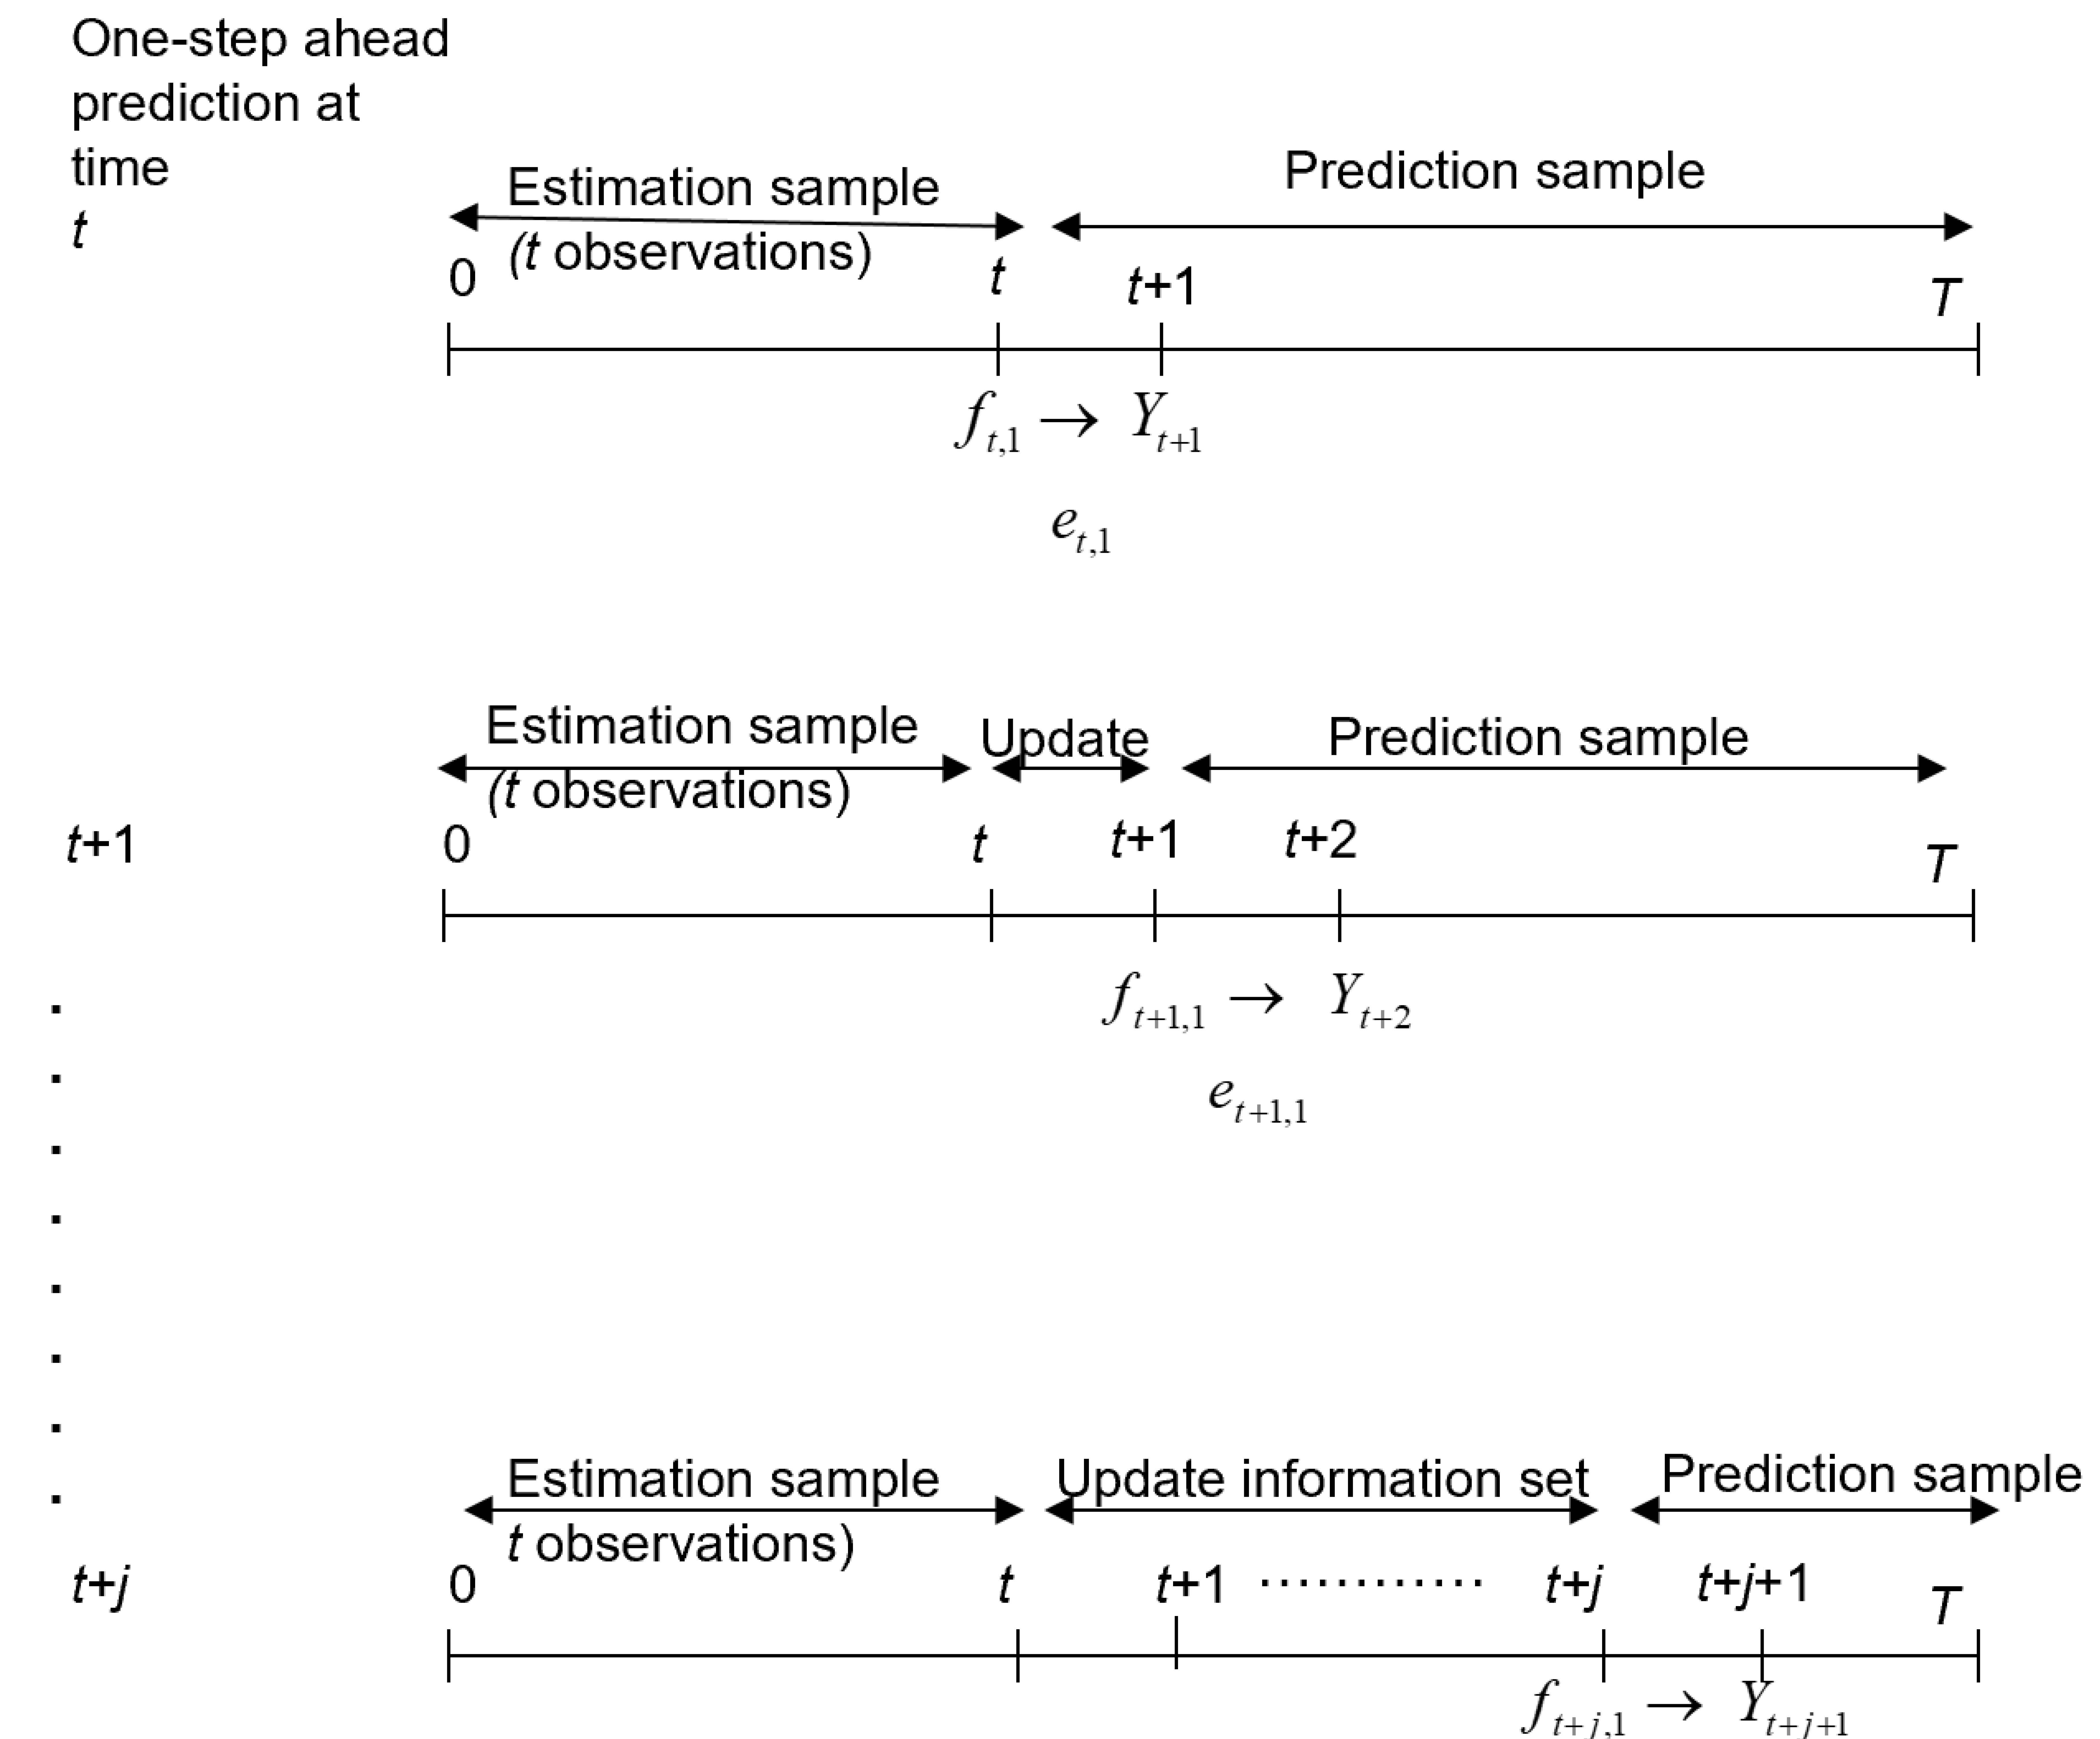
\includegraphics[width=0.5\linewidth]{figures/fixed_forecast}
				\caption{Fixed Forecasting Scheme}
			\end{figure}
	\subsection{Loss Function}
		\begin{definition}
			A loss function $L(e)$ is a real-valued function defined on the space of \emph{forecast errors}, $\mc{E}$, and satisfies the following properties
			\begin{enumerate}[(i)]
				\item $L(e) = 0 \iff ||e|| = 0$;
				\item $\forall e \in \mc{E}, L(e) \geq 0$\footnote{Since forecasting here can be considered as an optimization process, with $L$ as the objective function. It's fine for $L$ not satisfying the non-negativity condition. However, by convention, we assume $L$ to be non-negative.};
				\item $L$ is \emph{monotonically increasing} in the norm of forecast error.
			\end{enumerate}
		\end{definition}
		
		\begin{example}[Symmetric Loss Functions with $\mc{E} = \R$]
			\begin{align}
				L(e) = a e^2,\ a > 0 \\
				L(e) = a |e|,\ a > 0
			\end{align}
		\end{example}
		
		\begin{example}[Asymmetric Loss Functions with $\mc{E} = \R$]
			\begin{align}
				L(e) = exp(ae) - ae - 1,\ a > 0 & \tx{ Linex Function} \\
				L(e) = a\ |e|\ \mathbb{I}(e \geq 0) + b\ |e|\ \mathbb{I}(e < 0) &\tx{ Lin-lin Function}
			\end{align}
		\end{example}
		
	\subsection{Optimal Forecast}
		\begin{definition}
			Based on information set $I_t$, the optimal forecast for future value $y_{t+h}$ is the $f^*_{t,h}$ minimize the \hl{expected loss function}
			\begin{equation}
				\expect{L|I_t} = \int L(y_{t+h} - \red{f_{t,h}}) f(y_{t+h})\ dy_{t+h}
			\end{equation}
		\end{definition}
		
		\begin{assumption}
			Assuming the forecast $f(y_{t+h}|I_t)$ follows
			\begin{equation}
				f(y_{t+h}|I_t) \sim \mc{N}(\expect{Y_{t+h}|I_t}, \var{Y_{t+h}|I_t})
			\end{equation}
		\end{assumption}
		
		\begin{proposition}
			Given symmetric quadratic $L$, the optimal forecast $f^*_{t,h}$ is 
			\begin{equation}
				\mu_{t+h|t} \equiv \expect{Y_{t+h}|I_t}
			\end{equation}
			\begin{proof}
				\begin{gather}
					\min_{f_{t, h} \in \R} L \equiv \int (y_{t+h} - f_{t, h})^2 f(y_{t+h}|I_t)\ dy_{t+h} \\
					\pd{L}{f_{t, h}} = -2 \int (y_{t+h} - f_{t, h}) f(y_{t+h}|I_t)\ dy_{t+h} = 0 \\
					\implies \int (y_{t+h} - f_{t, h}) f(y_{t+h}|I_t)\ dy_{t+h} = 0 \\
					\implies \int y_{t+h} f(y_{t+h}|I_t)\ dy_{t+h} = f_{t, h} \int  f(y_{t+h}|I_t)\ dy_{t+h} \\
					\implies f_{t, h} = \expect{y_{t+h}|I_t} \equiv \mu_{t+h|t}
				\end{gather}
			\end{proof}
		\end{proposition}
		
	\section{Moving Average Process}
\end{document}


























